\section{Brief introduction}
Modeling is a powerful tool in synthetic biology and engineering. Mmodeling has provided us with an important engineering approach to characterize our pathways and predict their performance, thus helped us with modifying and testing our designing.

Through our model, we hope to gain insight of the gene expression dynamics of our whole circuit. And also we tried to better characterize our parts, analyze our experimental data,and protein transport and concentration changes throughout the whole process. Several tools including ODEs and interpolation are employed.


\section{Kinetic model}
\subsection{analysis of the problem}

\begin{figure}[h]
\centering
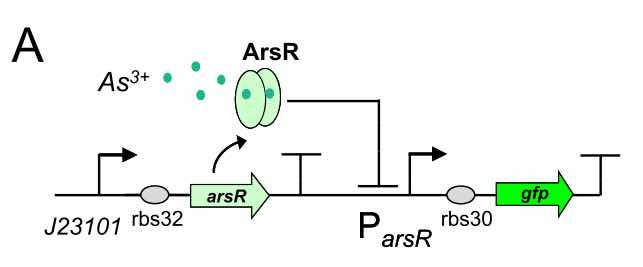
\includegraphics[width=12cm,height=5cm]{1}
\caption{Schematic diagram of plasmid1}
\end{figure}

At the beginning, on the plasmid1, the promoter $P_{arsR}$ isn't bound with ArsR, and thus active. And ArsR and $smURFP_l$ are transcribed from the promoter $P_{arsR}$. $smURFP_l$ means leaking expression without the expression of $As^{3+}$.Then ArsR will bind with the promoter $P_{arsR}$ and make it inactive. 

\begin{equation}
P_{J23104} \stackrel{k_1}{\longrightarrow} P_{J23104}+ArsR
\end{equation}

\begin{equation}
P_{arsR} \stackrel{k_2}{\longrightarrow} P_{arsR} +smURFP
\end{equation}

\begin{equation}
ArsR+P_{arsR} \xrightleftharpoons[k_{-3}]{k_3}ArsR*P_{arsR} 
\end{equation} 

On the plasmid 2, fusion protein of dcas9(dead Cas9, a mutant of Cas9) and RNAP(RNA polymerase) are produced after transcription.

\begin{equation}
P_{tet} \stackrel{k_{4}}{\longrightarrow} P_{tet} +dCas9-RNAP
\end{equation}

\begin{equation}
P_{tet} \stackrel{k_{5}}{\longrightarrow} P_{tet} +sgRNA
\end{equation}

\begin{figure}[h]
	\centering
	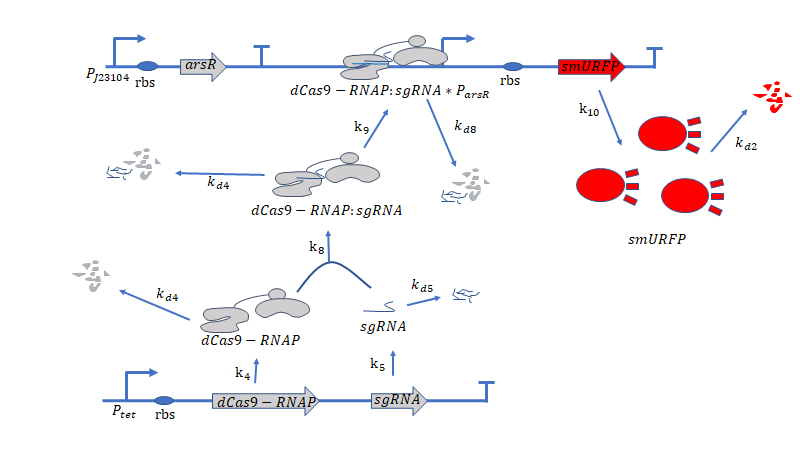
\includegraphics[width=12cm,height=5cm]{2}
	\caption{Schematic diagram of dCas9/RNAP}
\end{figure}

dCas9/RNAP can bind with it's target DNA sequence(upstream of promoter sequence) but not cut it. Simultaneously, dCas9 should have led RNAP to bind to the promoter $P_{arsR_d}$ and enhanced the transcription of GFP. However, the promoter $P_{arsR}$ has already bound with ArsR, as a result, RNAP can't bind with the promoter $P_{arsR}$ . \\ 

However, at the presence of $As^{3+}$, $As^{3+}$ can bind with ArsR, then dissociate ArsR and $P_{arsR_d}$, and combine RNAP and $P_{arsR_d}$. \\

(Declaration: $[dCas9/RNAP] = [dCas9] = [RNAP]$ ; $[P_{arsR_d}] = [P_{arsR_u}] = \frac{1}{2}[P_{arsR}]$ )

\begin{equation}
ArsR +As^{3+}\xrightleftharpoons[k_{-6}]{k_6}As^{3+}*ArsR
\end{equation}

\begin{equation}
ArsR*P_{arsR} +As^{3+}\xrightleftharpoons[k_{-7}]{k_7}P_{arsR}+ As^{3+}*ArsR
\end{equation}

\begin{equation}
dCas9-RNAP+sgRNA\xrightleftharpoons[k_{-8}]{k_8} dCas9-RNAP:sgRNA
\end{equation}

\begin{equation}
dCas9-RNAP:sgRNA+P_{arsR}\xrightleftharpoons[k_{-9}]{k_9} dCas9-RNAP:sgRNA*P_{arsR}
\end{equation}

\begin{equation}
dCas9-RNAP:sgRNA*P_{arsR}\stackrel{k_{10}}{\longrightarrow} dCas9-RNAP:sgRNA*P_{arsR}+smURFP
\end{equation}
\\\\
Take the degration into account
\\\\
\begin{equation}
ArsR\stackrel{k_{d1}}{\longrightarrow}Ø
\end{equation}

\begin{equation}
smURFP\stackrel{k_{d2}}{\longrightarrow}Ø
\end{equation}


\begin{equation}
ArsR*P_{arsR}\stackrel{k_{d3}}{\longrightarrow}P_{arsR}
\end{equation}

\begin{equation}
As^{3+}*ArsR\stackrel{k_{d4}}{\longrightarrow}As^{3+}
\end{equation}

\begin{equation}
dCas9-RNAP\stackrel{k_{d5}}{\longrightarrow}Ø
\end{equation}

\begin{equation}
sgRNA\stackrel{k_{d6}}{\longrightarrow}
\end{equation}

%\begin{equation}
%dCas9-RNAP:sgRNA\stackrel{k_{d7}}{\longrightarrow}dCas9-RNAP
%\end{equation}

\begin{equation}
dCas9-RNAP:sgRNA\stackrel{k_{d7}}{\longrightarrow}Ø
\end{equation}

%\begin{equation}
%dCas9-RNAP:sgRNA*P_{arsR}\stackrel{k_{d8}}{\longrightarrow}dCas9-RNAP+P_{arsR}
%\end{equation}

\begin{equation}
dCas9-RNAP:sgRNA*P_{arsR}\stackrel{k_{d8}}{\longrightarrow}P_{arsR}
\end{equation}
\\\\
\begin{table}[htbp]
	\centering
	\caption{\label {tab:test} Parameters}
	\begin{tabular}{cccccccccccccccccc}
		\toprule
		Rate constants & Value& units \\
		\midrule
		k1 & 1.999e-5 &1/s \\
		k2 & 3.312e-6 &1/s \\
		k3 & 3.3e7    & 1/M    \\
		k4 &1.995e-5 &1/s\\
		k5 & 3.312e-6 &1/s \\
		k6 &1.66e7   &1/M  \\
		k7  &1.26e4 &1/s  \\
		k8&1.6e-2& 1/s\\
		k9 &1.66e-5&1/s\\ 
		k10&4e-5&1/s\\
		kd1 & 3.07e-3&1/s\\
		kd2&1e-5&1/s\\
		kd3&1e-3&1/s\\
		kd4&1.53e-3&1/s\\
		kd5 & 2e-2&1/s\\
		kd6&7.62e-3&1/s\\
		kd7& 1e-2&1/s\\
		kd8&1e-1&1/s\\		
		\bottomrule
	\end{tabular}
\end{table}



\subsection{simulation }
\begin{figure}[h]
	\centering
	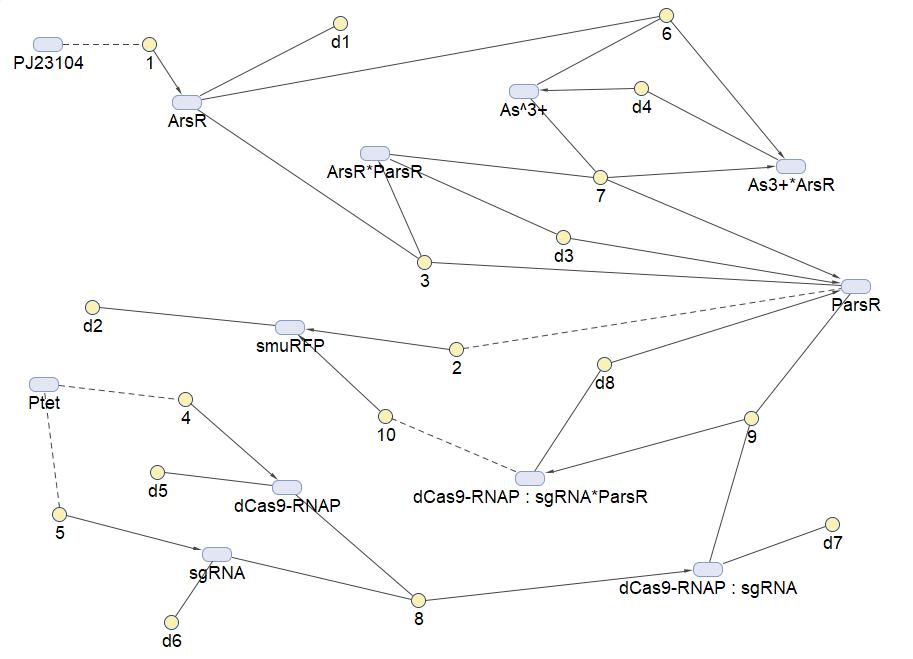
\includegraphics[width=10cm,height=7cm]{screenshot003}	
	\caption{reaction map generated from the reaction set above using SimBiology Toolbox}
\end{figure}
SimBiology toolbox provides functions for modeling, simulating, and analyzing biochemical pathways on basis of the powerful computing engine of Matlab.

\begin{figure}[h]
	\centering
	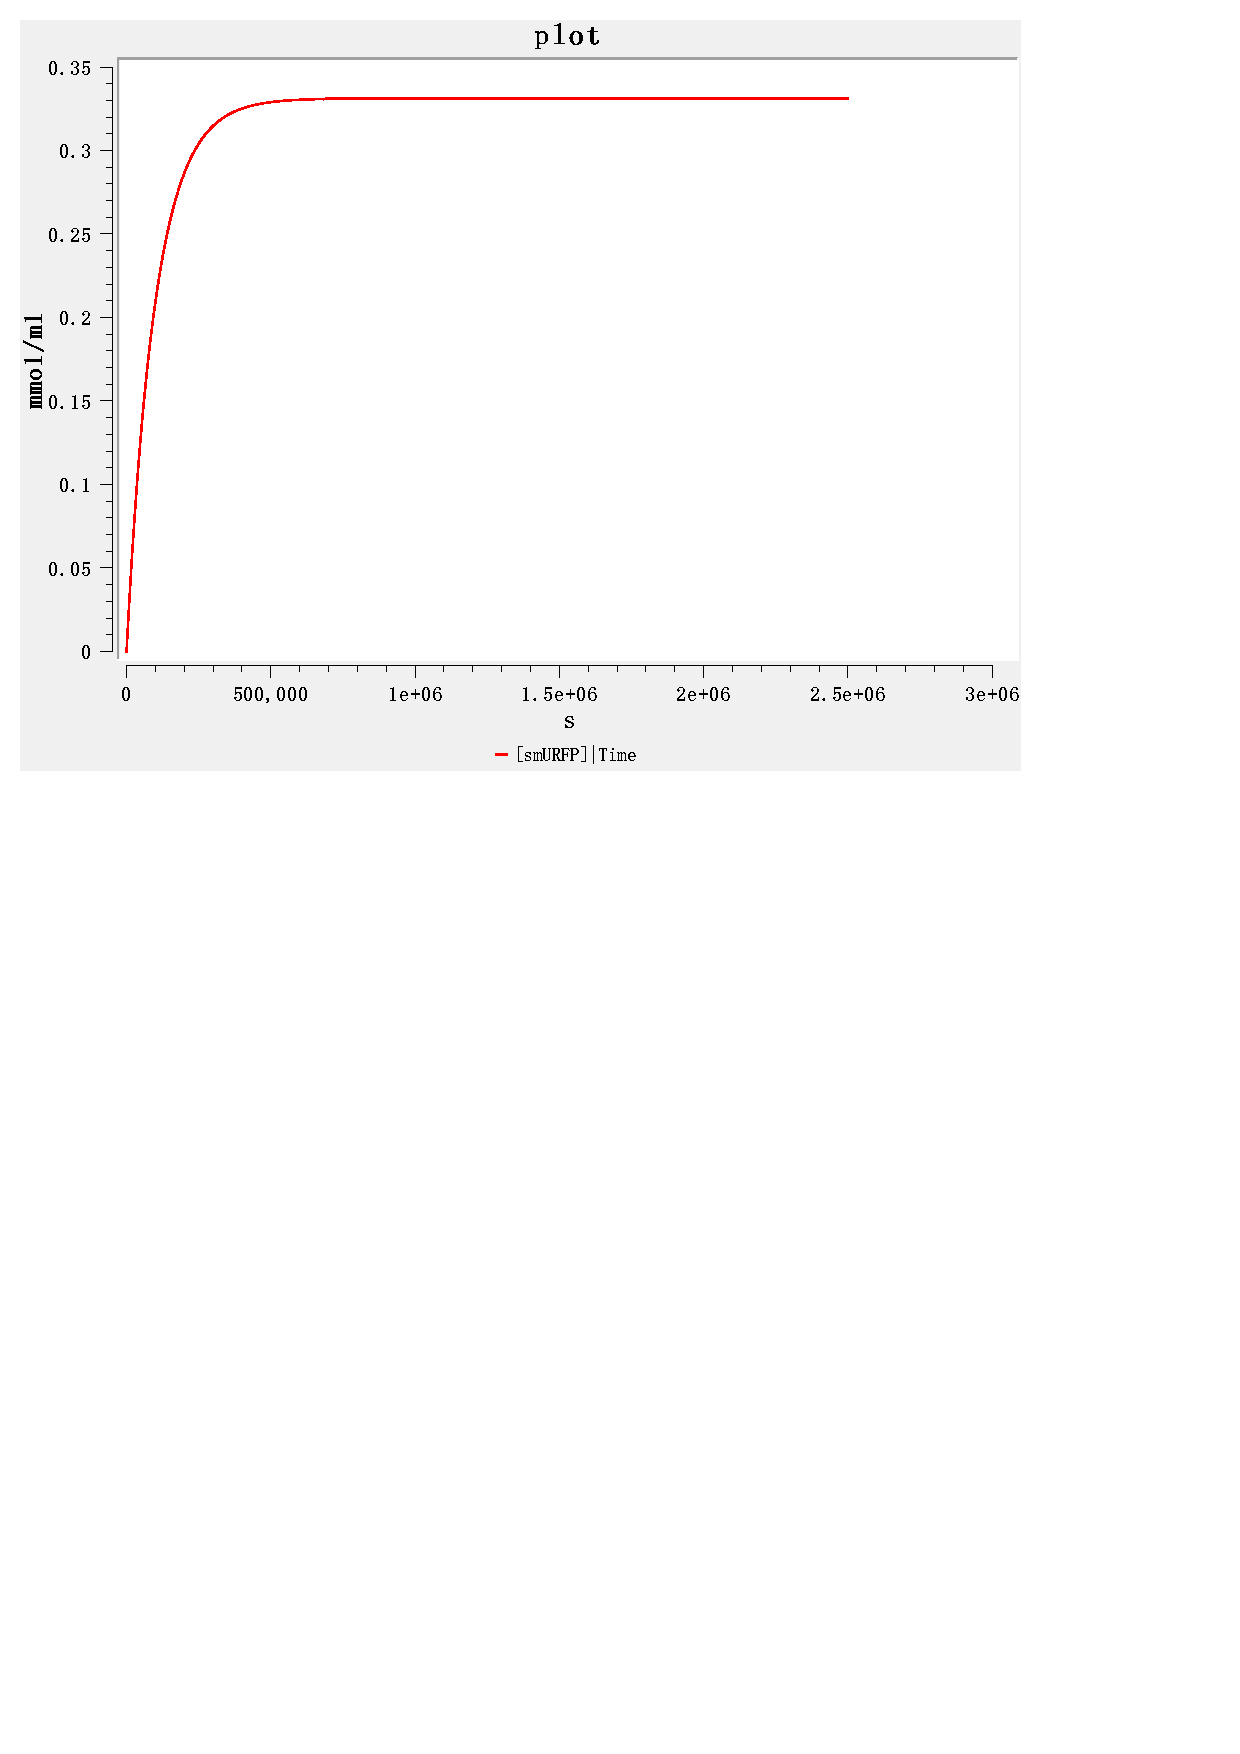
\includegraphics[width=10cm,height=10cm]{smuRFP}
	\caption{Schematic diagram of smURFP fluorescence by COPASI}
\end{figure}



COPASI is freeware developed withcollaboration of VBI and EMLR. It provides
almost the same functions as SimBiology, though not quite powerful. But compared with SimBiology, it provides a friendly user interface for model analysis, such as parameter estimation,and parameter scan.

Through the figure, we can see that the smURFP fluorescence gradually increased and then reached a steady state after a period of time  in the presence of arsenic ions.

\section{References} 
1.Berset, Y. et al. Mechanistic Modeling of Genetic Circuits for ArsR Arsenic Regulation. ACS Synthetic Biology 6, 862–874 (2017).\\

2.Bikard, D.et al. Programmable repression and activation of bacterial gene expression using an engineered CRISPR-Cas system. Nucleic Acids Research 41, 7429–7437 (2013).\\

3.Cai, Y. et al. Modeling the arsenic biosensor system. BMC Systems Biology 1, P83 (2007).\\

4.Pola-López, L. A. et al. Novel arsenic biosensor “POLA” obtained by a genetically modified E. coli bioreporter cell. Sensors and Actuators B: Chemical 254, 1061–1068 (2018).

\end{document}






